\documentclass[12pt]{article}

\usepackage{float}
\usepackage[pdftex]{graphicx} 
\graphicspath{{../img/}}
\DeclareGraphicsExtensions{.pdf,.jpeg,.png,.jpg} 

\usepackage{listings}
\lstset{language=Python, keywordstyle=\color{blue}, stringstyle=\color{olive}, breaklines=true, showstringspaces=false, float, tabsize=2}
\usepackage{xcolor}
\usepackage{textcomp}
\usepackage{subcaption}
\usepackage{amsmath}

%opening
\title{Laboratory exercise no. 5: Application of box models to Upper Danube catchment simulation}
\author{Piotr Gawry\'s $<pgawrys2@gmail.com>$}

\begin{document}

\maketitle

\section{Introduction}
The goal of this laboratory is to implement simulation capable of calculating a mean residence time of water in the Upper Danube. In the simulation we will use exponential transit time distribution function, practice calculating integrals programmatically, learn about box models and explore two methods of finding optimal parameters.

\subsection{Mathematical Model}

To calculate a mean residence time of water we are going to use mathematical model shown in the equation below:

\begin{equation} \label{eq:1}
C(t) = \int_{- \infty}^{t} C_{in}(t') \cdot g(t - t') \cdot exp[-\lambda \cdot (t - t')] \cdot dt'
\end{equation}
Where:
\begin{itemize}
	\item $C(t)$ -- output function.
	\item $C_{in}(t')$ -- input function.
	\item $g(t - t')$ -- transit time distribution function.
	\item $\lambda = 4.696 * 10^{-3}$ -- radioactive decay constant (tritium).
	\item t -- time variable.
	\item t' -- integration parameter.
\end{itemize}

One more important thing to note is that model used in this exercise is considered as \textit{box model}. This means that the modelled object is treated as \textit{black-box} -- we reason about it solely on the basis to its response to given inputs. Concentration of the tracer in the precipitation is used as an input and the concentration of the tracer is the output.

\subsection{Data for modelling}

The input data is delivered in "opady.prn" file which contains mean amount of tritium in the precipitations during given time. There is also second file -- "dunaj.prn" containing real measurements which will be used to validate our model. Those are illustrated on Figure ~\ref{dane}.

\begin{figure}[H]
	\centering
	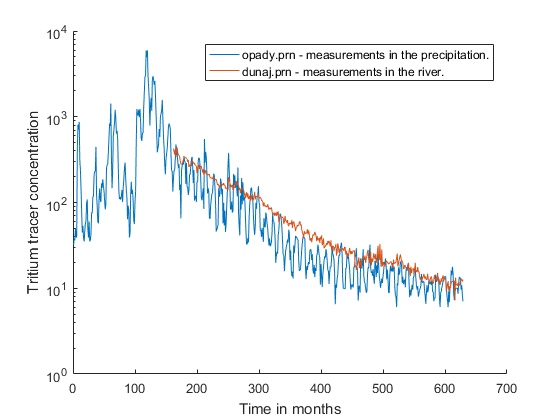
\includegraphics[width=\textwidth]{dane}
	\caption{Measurements of tritium concentration in the precipitation and in Danube river.}    
	\label{dane}
\end{figure}

\section{Simulation}

\subsection{Calculating convolution integral}
First step to implement discussed model is to calculate the convolution integral for selected transit time distribution function. During this laboratory we decided to choose \textbf{exponential model} which is expressed as follows:

\begin{equation}
g(t - t') = {t^{-1}}_t \cdot exp(-(t - t')/t_t)
\end{equation}

Simple way to actually write it in Matlab is substituting $g(t - t')$ in the equation ~\ref{eq:1} and executing it in loop to reflect integral. Function representing this equation can be found at the end of report in subsection ~\ref{code:convInt}. 

One of the variables \textbf{tt} (to denote $t_t$) is mean residence time. It is taken as a parameter to function but it's missing. In the next sections we will explore two methods to acquire this value and compare them.

\subsection{Mean residence time using trial-error method}

One of the methods to derive \textbf{tt} is called \textbf{trial-error method}. The way it works is that we calculate Root Mean Squared Error and take successive \textbf{tt} values while error is decreasing, otherwise we stay with last value. To calculate Root Mean Squared Error we need to have some results to compare and those are fortunately available in "dunaj.prn" file. The implementation is provided in section ~\ref{code:trialError}. 

In this model I chose to check possible values from $t_t = 1$ and it resulted in \textbf{$t_t = 8$} using step = 1. After tuning it to 0.001 it took significantly more time (minutes instead of seconds) but allowed to find more precise value of mean residence time which was \textbf{7.241}. 

While this approach works for this use case there is a danger with this method - if we were to choose different range of values we could get different answer. This is easy to see on the figure ~\ref{meanSquare} where we can see that the result would be much different for higher initial $t_t$. For instance if we were to choose range from 150 to 300 the minimal mean residence would be something around 210.

\begin{figure}[H]
	\centering
	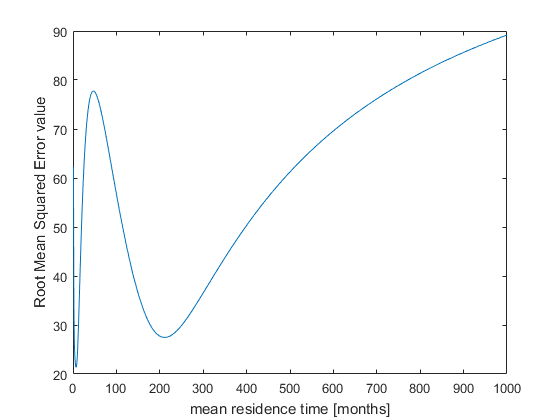
\includegraphics[width=\textwidth]{meanSquare}
	\caption{Relation of Root Mean Squared Error to different $t_t$ values}
	\label{meanSquare}
\end{figure}

Furthermore, this implementation is not ideal because it could go wrong for small oscillations in Root Mean Squared Error missing proper minimums.

\subsection{Mean residence time using objective function}

There is other approach which is included in the report. Instead of searching for optimal $t_t$ value looping through results manually we can use MATLAB's \textbf{fminunc} function which is going to find the value of the local minima manually. Code can be found in the subsection ~\ref{code:objective}. There are two snippets -- \textbf{fminunc} requires taking function as a parameter and MATLAB version which was used to do this report doesn't allow having functions in script file.

The result was \textbf{7.2401} and the execution time was much faster than in case of manual approach as presented in previous section.

\subsection{Comparison}

Both trial-error method and using MATLAB's built in function provided similar results, 7.241 and 7.2401 respectively. Trial-error method could probably provide the same result with even lower time step but it would approach tens of minutes of execution time in comparison to seconds for \textit{fminunc}. In case of this simulation the former time could be feasible but it is easy to imagine use case with much more variables leading to serious performance problems.

What's more it is probably better to use proven built in functions instead of implementing everything yourself which can lead to errors and sub-optimal solutions.

\begin{figure}[H]
	\centering
	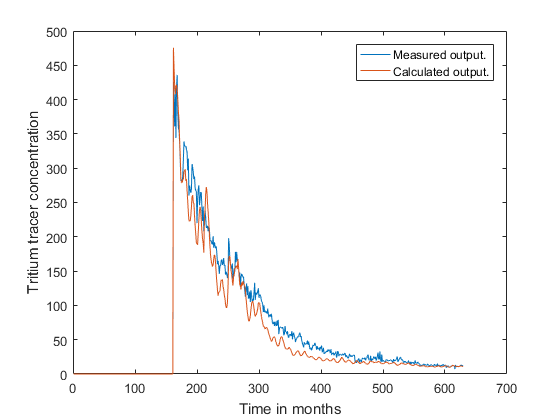
\includegraphics[width=\textwidth]{finalPlot}
	\caption{Amount of tritium in Danube river for mean residence time of water = 7.24 in comparison to real measurements.}
\end{figure}

\section{Conclusion}

Over the course of this classes we implemented integral equation using exponential transit time distribution function and then used both trial-error and inverse modelling method learning about dangers coming from using manually implemented methods.

Implemented code allowed us to calculate a mean residence time of water for tritium tracer in Upper Danube. Using a mean value of tritium concentration in the precipitation as input data we came very close to real measurements.

\section{Appendix -- Source Code}
\subsection{Plotting opady.prn and dunaj.prn}
\lstinputlisting[language=Matlab,frame=single]{../source_code/plotData.m}
\subsection{Convolution integral using exponential model}
\label{code:convInt}
\lstinputlisting[language=Matlab,frame=single]{../source_code/convInt.m}
\subsection{Trial-error method}
\label{code:trialError}
\lstinputlisting[language=Matlab,frame=single]{../source_code/trialError.m}
\subsection{Objective function}
\label{code:objective}
\lstinputlisting[language=Matlab,frame=single]{../source_code/objectiveMain.m}
\lstinputlisting[language=Matlab,frame=single]{../source_code/objective.m}
\subsection{Final plot}
\label{code:finalPlot}
\lstinputlisting[language=Matlab,frame=single]{../source_code/plotDataComp.m}

\end{document}
